
\hypertarget{cv:registrarPExt}{\section{Registrar Término de Glosario}} \label{sec:registrarPExt}

	Esta funcionalidad le permitirá registrar un punto de extensión dentro del caso de uso que se esta operando. 

		\subsection{Procedimiento}

			%Pasos de procedimiento
			\begin{enumerate}
	
			\item Oprima el botón \IURegistrar{} de la pantalla \ref{fig:GestionarPuntosExt} ''Gestionar Puntos de Extensión''.
			
			\item Se mostrará la pantalla \ref{fig:registrarPExt} ''Registrar Punto de Extensión''.

			%Pantalla
			\begin{figure}[H]
				\begin{center}
					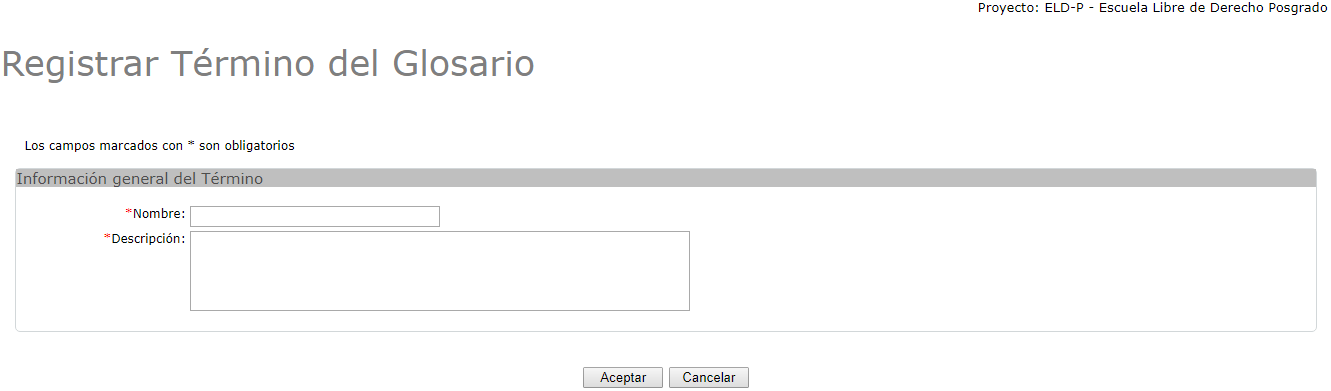
\includegraphics[scale=0.5]{roles/lider/glosario/pantallas/IU6-1registrarTermino}
					\caption{Registrar Punto de Extensión}
					\label{fig:registrarPExt}
				\end{center}
			\end{figure}
		
			\item Elija el caso de uso al que extenderá el punto, ingrese la causa y en que región de la trayectoria pasa esto.
			
			\item En la región de la trayectoria usted podrá referenciar algunos tipos de elementos que se encuentren registrados dentro del proyecto actual, mendiante los siguientes TOKENS:
			
			\begin{itemize}
				\item Podrá referenciar elementos de tipo trayectoria con el TOKEN: ''TRAY·''.
				\item Podrá referenciar elementos de tipo paso con el TOKEN: ''P·''.
			\end{itemize}
			
			\item Oprima el botón \IUAceptar.
			
			\item Se mostrará el mensaje \ref{fig:pextRegistrado} en la pantalla \ref{fig:GestionarPuntosExt} ''Gestionar Puntos de Extensión''.
			
			\begin{figure}[htbp!]
				\begin{center}
					
\includegraphics[scale=0.5]{roles/lider/glosario/pantallas/IU6-1MSG1}
					\caption{MSG: Punto de Extensión Registrado}
					\label{fig:pextRegistrado}
				\end{center}
			\end{figure}
			\end{enumerate}